%\VignetteIndexEntry{Using StardogR}
\documentclass{article}\usepackage[]{graphicx}\usepackage[]{xcolor}
% maxwidth is the original width if it is less than linewidth
% otherwise use linewidth (to make sure the graphics do not exceed the margin)
\makeatletter
\def\maxwidth{ %
  \ifdim\Gin@nat@width>\linewidth
    \linewidth
  \else
    \Gin@nat@width
  \fi
}
\makeatother

\definecolor{fgcolor}{rgb}{0.345, 0.345, 0.345}
\newcommand{\hlnum}[1]{\textcolor[rgb]{0.686,0.059,0.569}{#1}}%
\newcommand{\hlstr}[1]{\textcolor[rgb]{0.192,0.494,0.8}{#1}}%
\newcommand{\hlcom}[1]{\textcolor[rgb]{0.678,0.584,0.686}{\textit{#1}}}%
\newcommand{\hlopt}[1]{\textcolor[rgb]{0,0,0}{#1}}%
\newcommand{\hlstd}[1]{\textcolor[rgb]{0.345,0.345,0.345}{#1}}%
\newcommand{\hlkwa}[1]{\textcolor[rgb]{0.161,0.373,0.58}{\textbf{#1}}}%
\newcommand{\hlkwb}[1]{\textcolor[rgb]{0.69,0.353,0.396}{#1}}%
\newcommand{\hlkwc}[1]{\textcolor[rgb]{0.333,0.667,0.333}{#1}}%
\newcommand{\hlkwd}[1]{\textcolor[rgb]{0.737,0.353,0.396}{\textbf{#1}}}%
\let\hlipl\hlkwb

\usepackage{framed}
\makeatletter
\newenvironment{kframe}{%
 \def\at@end@of@kframe{}%
 \ifinner\ifhmode%
  \def\at@end@of@kframe{\end{minipage}}%
  \begin{minipage}{\columnwidth}%
 \fi\fi%
 \def\FrameCommand##1{\hskip\@totalleftmargin \hskip-\fboxsep
 \colorbox{shadecolor}{##1}\hskip-\fboxsep
     % There is no \\@totalrightmargin, so:
     \hskip-\linewidth \hskip-\@totalleftmargin \hskip\columnwidth}%
 \MakeFramed {\advance\hsize-\width
   \@totalleftmargin\z@ \linewidth\hsize
   \@setminipage}}%
 {\par\unskip\endMakeFramed%
 \at@end@of@kframe}
\makeatother

\definecolor{shadecolor}{rgb}{.97, .97, .97}
\definecolor{messagecolor}{rgb}{0, 0, 0}
\definecolor{warningcolor}{rgb}{1, 0, 1}
\definecolor{errorcolor}{rgb}{1, 0, 0}
\newenvironment{knitrout}{}{} % an empty environment to be redefined in TeX

\usepackage{alltt}

\usepackage{hyperref}
\usepackage{parskip}
\usepackage{graphicx}
\usepackage[utf8]{inputenc}



\title{Using StardogR}
\author{Catherine Dalzell}
\date{2023-05-12}
\IfFileExists{upquote.sty}{\usepackage{upquote}}{}
\begin{document}
\maketitle

\tableofcontents




\begin{knitrout}
\definecolor{shadecolor}{rgb}{0.969, 0.969, 0.969}\color{fgcolor}\begin{kframe}
\begin{alltt}
\hlkwd{library}\hlstd{(}\hlstr{'stardogR'}\hlstd{)}
\hlkwd{library}\hlstd{(}\hlstr{'purrr'}\hlstd{)}
\hlkwd{library}\hlstd{(}\hlstr{'jsonlite'}\hlstd{)}
\hlkwd{library}\hlstd{(}\hlstr{'httr'}\hlstd{)}
\end{alltt}
\end{kframe}
\end{knitrout}


\section{Stardog and R}

Stardog is both an Enterprise graph database and a knowledge graph, capable of integrating diverse data sources. Stardog can materialize data to RDF format and query those data using the Sparql query language. Queries can also be made through Stardog against other data sources that have been mapped to semantic concepts Stardog can use. Stardog can thus function as a portal that unifies external data sources, as a standalone database in its own right, and as a combination of these things. A Stardog database can also access the growing number of public RDF data sources.

Stardog supports an \href{https://stardog-union.github.io/http-docs/}{HTTP API}. For each of use, wrappers have been written to this API for an assortment of programming languages. \tt{stardogR} provides an R wrapper for those portions of the API most likely to be used by Data Scientists and Statisticians.

\subsubsection*{Remark}
The Stardog API provides a full suite of tools for managing the database and querying its contents. There are commands for creating users with different roles and permissions; creating the database and setting its properties; loading data; connecting to other data sources; managing meta-data; using Graphql; managing named graphs and issuing Sparql queries. Currently, \tt{stardogR} implements those commands most likely to be of interest to Data Scientists. Additional wrappers may be added in future versions.

\subsection{An R workflow}

Data scientists are used to working with more than one tool. At a minimum, there is a database of some kind for storing and organizing large quantities of data, and an analytic tool such as R. A good query language can explore the data and return useful summaries, however there usually comes a point where a tool with more finesse is required, such as R. This is also the point at which the analyst risks losing control of the process. The query is written in one language and the analysis is written in another. The analysis depends upon the results of the query, but that piece may not be in the analytic record. With \tt{stardogR}, queries and machine learning can both be done from an RMarkdown document or R notebook, thus ensuring complete reproducibility.



\section{The Toronto Beaches data}

\tt{stardogR} comes with a set of data drawn from the open data portal of the City of Toronto. This set contains daily readings of eColi levels at each of Toronto's public beaches over the summer months of 2007 through 2013.

\begin{verbatim}
>data('beaches', package = 'stardogR')
>names(beaches)
[1] "Beach_ID"       "Beach_Name"     "Sample_Date"
[4] "Publish_Date"   "eColi_Level"    "Beach_Status"
[7] "Beach_Advisory"
\end{verbatim}

Each row contains the results of one eColi sample. We have the eColi measurement, the name and ID of the beach where there the measurement was taken, sample and publication date (typically the same day) and the beach status. Status is recorded in two columns: a simple label in \tt{Beach\_Status}, like SAFE or UNSAFE, and a more detailed description in \tt{Beach\_Advisory}.  The beach is considered to be unsafe when the eColie measurement goes above 100.


\section{Building the database}

To run these examples, you first need access to a Stardog server. Every interaction with Stardog requires the endpoint of the installation, a username and a password. For convenience, these are stored in a data structure of class stardog.

\subsection{The Stardog data structure}

\begin{knitrout}
\definecolor{shadecolor}{rgb}{0.969, 0.969, 0.969}\color{fgcolor}\begin{kframe}
\begin{alltt}
\hlstd{sg} \hlkwb{<-} \hlkwd{Stardog}\hlstd{(}\hlstr{"http://localhost:5820"}\hlstd{,} \hlstr{"admin"}\hlstd{,} \hlstr{"admin"}\hlstd{,} \hlkwc{encoding} \hlstd{=} \hlstr{"UTF-8"}\hlstd{)}
\end{alltt}
\end{kframe}
\end{knitrout}

The default username and password for a local installation are \tt{admin} and \tt{admin}. Object \tt{sg} holds the connection information. Replace these values with our own endpoint and authorization strings. Argument \tt{encoding} defaults to UTF-8

The stardog object is also used to hold transaction id's, the name of the active database and other information. In a typical object oriented language (which R is not), all subsequent functions would be methods against the stardog object and the class members would be private. In \tt{stardogR}, the Stardog API is expressed as a collection of functions taking a stardog object as their first argument.

\bf{Warning:} Since the stardog object is a simple S3 class, the user could change its values at will. I suggest against doing so. There are functions for accessing and changing the class values. The \tt{print} method for class stardog hides most of the data in the object.

Note that the stardog object does not touch the database. It does not check if the database is online or whether the credentials are valid. It simply creates a data structure for holding that information.

\subsection{Selecting a database}

Working with data requires a database. In the typical, Enterprise scenario, the database already exists and we just need to add its name to the stardog object. However, in a development setting, we might well need to create a database, or reset an existing one (i.e. delete and recreate), for model building or a proof of concept. Function \tt{use\_database} can handle all of these scenarios.

\bf{Use an existing database}

\begin{knitrout}
\definecolor{shadecolor}{rgb}{0.969, 0.969, 0.969}\color{fgcolor}\begin{kframe}
\begin{alltt}
\hlstd{sg} \hlkwb{<-} \hlkwd{use_database}\hlstd{(sg,} \hlkwc{dbName} \hlstd{=} \hlstr{"myDB"}\hlstd{)}
\end{alltt}
\end{kframe}
\end{knitrout}

\bf{Create a new database and use it}

\begin{knitrout}
\definecolor{shadecolor}{rgb}{0.969, 0.969, 0.969}\color{fgcolor}\begin{kframe}
\begin{alltt}
\hlstd{sg} \hlkwb{<-} \hlkwd{use_database}\hlstd{(sg,} \hlkwc{dbName} \hlstd{=} \hlstr{"myDB"}\hlstd{,} \hlkwc{create} \hlstd{=} \hlnum{TRUE}\hlstd{)}
\end{alltt}
\end{kframe}
\end{knitrout}

\bf{Drop and recreate a new database and use it}

\begin{knitrout}
\definecolor{shadecolor}{rgb}{0.969, 0.969, 0.969}\color{fgcolor}\begin{kframe}
\begin{alltt}
\hlstd{sg} \hlkwb{<-} \hlkwd{use_database}\hlstd{(sg,} \hlkwc{dbName} \hlstd{=} \hlstr{"myDB"}\hlstd{,} \hlkwc{reset} \hlstd{=} \hlnum{TRUE}\hlstd{)}
\end{alltt}
\end{kframe}
\end{knitrout}

The function requires that you be explicit about your intentions. You can't delete an existing database without \tt{reset = TRUE}.

Since R is a functional language that avoids side effects, the stardog object is not updated within the function. It is returned and needs to be assigned to something if we want to use the database. If the call was to create or reset a database, that particular side effect will occur in the Stardog database, but the stardog object with the database name must be assigned, as shown in the examples.

Sometimes, we may want to reset the database slot to NA, in which case, we can run:

\begin{knitrout}
\definecolor{shadecolor}{rgb}{0.969, 0.969, 0.969}\color{fgcolor}\begin{kframe}
\begin{alltt}
\hlstd{sg} \hlkwb{<-} \hlkwd{use_database}\hlstd{(sg,} \hlkwc{dbName} \hlstd{=} \hlstr{"myDB"}\hlstd{,} \hlkwc{set_to_NA} \hlstd{=} \hlnum{TRUE}\hlstd{)}
\end{alltt}
\end{kframe}
\end{knitrout}

This call makes no changes to the Stardog database.

\subsection{Adding data}

\tt{stardogR} allows adding data in three days.

\begin{itemize}
  \item Add RDF triples to the database
  \item Add the contents of an R DataFrame, using a mapping file
  \item Run an insert query to add triples based on data already present in the database.
\end{itemize}

The following code snippet shows how one might reset a database for the Toronto beaches data, load the data and add the ontology. The beaches data is included in the packages. For the mapping and onto strings, use the values developped in vignette \it{usingStarmap}


Now, build the database locally or against your own endpoint.

\begin{knitrout}
\definecolor{shadecolor}{rgb}{0.969, 0.969, 0.969}\color{fgcolor}\begin{kframe}
\begin{alltt}
\hlstd{sg} \hlkwb{<-} \hlkwd{Stardog}\hlstd{(}\hlstr{"http://localhost:5820"}\hlstd{,} \hlstr{"admin"}\hlstd{,} \hlstr{"admin"}\hlstd{)}
\hlstd{sg} \hlkwb{<-} \hlkwd{use_database}\hlstd{(sg,} \hlstr{"beaches"}\hlstd{,} \hlkwc{create} \hlstd{=} \hlnum{TRUE}\hlstd{)}
\hlkwd{add_namespace}\hlstd{(sg,} \hlkwc{uri} \hlstd{=} \hlstr{"http://beach.stardog.com/"}\hlstd{,} \hlkwc{prefix} \hlstd{=} \hlstr{"beach"}\hlstd{)}
\hlkwd{add_dataframe}\hlstd{(sg, beaches,} \hlkwc{mapping} \hlstd{= mapping_string)}
\hlkwd{add_ttl}\hlstd{(sg,} \hlkwc{ttl} \hlstd{= onto_string,} \hlkwc{graph} \hlstd{=} \hlstr{"beach:onto"}\hlstd{)}
\hlkwd{query}\hlstd{(sg)}
\end{alltt}
\end{kframe}
\end{knitrout}

\begin{enumerate}
  \item Create the stardog object with localhost endpoint
  \item Update object \tt{sg} by adding the name of a database. Set \tt{create = TRUE} to crete. Use \tt{reset = TRUE} if the database already exists and you want a clean slate.
  \item Add a namespace. \tt{add\_namespace} can add one prefix-urn pair for each call. It checks if the namespace already exists.
  \item Add the beaches data from DataFrame \tt{beach}. The mapping file is supplied as a long string
  \item Add the ontology triples. The turtle formatted RDF is also in string format. In this example, I am adding the ontology to a named graph. Note that I am referring to the named graph using the namespace prefix previously defined.
  \item Run a query as a reality check. Function \tt{query} returns the number of triples in the database.
\end{enumerate}

The ontology and mappings can be generated using function \tt{starmap}, which is described in a different vignette.

\subsection{A quick plot of the ontology}

We can get a look at the ontology using function \tt{plotSchema}

\begin{knitrout}
\definecolor{shadecolor}{rgb}{0.969, 0.969, 0.969}\color{fgcolor}\begin{kframe}
\begin{alltt}
\hlkwd{plotSchema}\hlstd{(sg,} \hlstr{"beach:onto"}\hlstd{,} \hlkwc{datatypes} \hlstd{=} \hlnum{TRUE}\hlstd{)}
\end{alltt}
\end{kframe}
\end{knitrout}

\begin{figure}[htbp]
\centerline{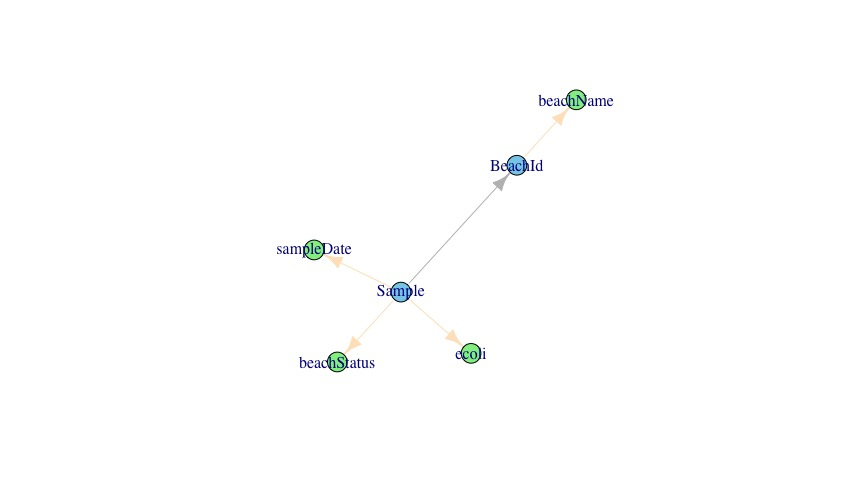
\includegraphics[scale = 0.5]{beachPlot.jpeg}}
\caption{Ontology plot for the Beaches data}
\label{fig}
\end{figure}

\section{Querying Stardog from R}

Sparql queries against Stardog can be simple requests for data, or they can effect change to the databases. \tt{stardogR} allows four kinds of query:

\begin{description}
  \item[ask] An ask query checks if certain patterns exist in the RDF and return true or false accordingly
  \item[construct] A construct query returns RDF triples, which could form the basis of a new graph. The construct query does not, in itself, change the existing database.
  \item[update] Update queries either insert or delete triples from the graph, depending on the key word in the query.
  \item[select] A select query returns an R DataFrame of results from the database.
\end{description}

\tt{stardogR} has one function, \tt{query}, for these use cases. It parses the supplied query to infer its type and takes appropriate action. It returns a DataFrame for a select query, a Boolean for an ask query, RDF for the construct query and a success message for an update.

\subsection{A select query}

A select query extracts data from the database and returns it as an R DataFrame.

\begin{knitrout}
\definecolor{shadecolor}{rgb}{0.969, 0.969, 0.969}\color{fgcolor}\begin{kframe}
\begin{alltt}
\hlstd{q} \hlkwb{<-} \hlstr{'
select ?beachName \{
  ?beach a beach:BeachId ;
    beach:beachName ?beachName .
\}
order by ?beachName
'}
\hlkwd{query}\hlstd{(sg,} \hlkwc{q} \hlstd{= q)}
\end{alltt}
\end{kframe}
\end{knitrout}

\begin{verbatim}
                      beachName
1          Bluffer's Beach Park
2           Centre Island Beach
3                  Cherry Beach
4         Gibraltar Point Beach
5          Hanlan's Point Beach
6               Kew Balmy Beach
7  Marie Curtis Park East Beach
8                   Rouge Beach
9               Sunnyside Beach
10    Sunnyside Enclosure Beach
11          Ward's Island Beach
12             Woodbine Beaches
\end{verbatim}

\subsubsection{Additional arguments}

Additional arguments can be supplied to the query function.

\begin{description}
  \item[limit] Number of lines of output to supply
  \item[reasoning] Boolean, used to switch on reasoning
  \item[graph] Issue the query against the named graph.
  \item[schema] Use the named reasoning schema
  \item[offset] Start the query this number of results in.
\end{description}

\tt{limit} and \tt{graph} can be included in the body of the query or supplied as arguments.

\begin{knitrout}
\definecolor{shadecolor}{rgb}{0.969, 0.969, 0.969}\color{fgcolor}\begin{kframe}
\begin{alltt}
\hlstd{q} \hlkwb{<-} \hlstr{'
select * \{?s ?p ?o .\}
'}
\hlkwd{query}\hlstd{(sg,} \hlkwc{q} \hlstd{= q,} \hlkwc{limit} \hlstd{=} \hlnum{5}\hlstd{)}
\end{alltt}
\end{kframe}
\end{knitrout}

\begin{verbatim}
     s                 p                  o
[1,] "beach:sample_1"  "beach:hasBeachId" "beach:beach_id_%20%20%20%20%20%20%20%20%201%20"
[2,] "beach:sample_12" "beach:hasBeachId" "beach:beach_id_%20%20%20%20%20%20%20%20%201%20"
[3,] "beach:sample_23" "beach:hasBeachId" "beach:beach_id_%20%20%20%20%20%20%20%20%201%20"
[4,] "beach:sample_34" "beach:hasBeachId" "beach:beach_id_%20%20%20%20%20%20%20%20%201%20"
[5,] "beach:sample_45" "beach:hasBeachId" "beach:beach_id_%20%20%20%20%20%20%20%20%201%20
\end{verbatim}

\subsection{An insert query}

The original data has a field called \tt{Beach\_Status}, which records SAFE or UNSAFE according as the eColi level is below 100 or not. Instead of importing that field, we can add it to the database with an insert query.

\begin{knitrout}
\definecolor{shadecolor}{rgb}{0.969, 0.969, 0.969}\color{fgcolor}\begin{kframe}
\begin{alltt}
\hlstd{q} \hlkwb{<-} \hlstr{'
insert \{
  ?sample beach:beachStatus ?status
\} where \{
  ?sample a beach:Sample ;
    beach:ecoli ?ecoli .
  BIND(IF(?ecoli < 100, "SAFE", "UNSAFE") as ?status)
\}
'}

\hlkwd{query}\hlstd{(sg, q)}
\end{alltt}
\end{kframe}
\end{knitrout}


And now, to check:

\begin{knitrout}
\definecolor{shadecolor}{rgb}{0.969, 0.969, 0.969}\color{fgcolor}\begin{kframe}
\begin{alltt}
\hlstd{q} \hlkwb{<-} \hlstr{'
select * \{
  ?sample beach:beachStatus ?status
\}
'}

\hlkwd{query}\hlstd{(sg, q,} \hlkwc{limit} \hlstd{=} \hlnum{5}\hlstd{)}
\end{alltt}
\end{kframe}
\end{knitrout}

\begin{verbatim}
     sample           status
[1,] "beach:sample_1" "SAFE"
[2,] "beach:sample_2" "SAFE"
[3,] "beach:sample_3" "SAFE"
[4,] "beach:sample_4" "SAFE"
[5,] "beach:sample_5" "SAFE"
\end{verbatim}

\subsection{Delete and insert into a named graph}

Adding statistics and derived quantities to the raw data is possibly not a \it{best practice}. Better is to add derived values to a named graph so they remain distinct from the original data set. Let's delete the previous insertion and then add the \tt{status} values to their own graph.

\begin{knitrout}
\definecolor{shadecolor}{rgb}{0.969, 0.969, 0.969}\color{fgcolor}\begin{kframe}
\begin{alltt}
\hlstd{q} \hlkwb{<-} \hlstr{'
delete \{
  ?sample beach:beachStatus ?status
\} where \{
  ?sample beach:beachStatus ?status .
\}
'}

\hlkwd{query}\hlstd{(sg, q)}
\end{alltt}
\end{kframe}
\end{knitrout}


reality check:

\begin{knitrout}
\definecolor{shadecolor}{rgb}{0.969, 0.969, 0.969}\color{fgcolor}\begin{kframe}
\begin{alltt}
\hlstd{q} \hlkwb{<-} \hlstr{'
select * \{
  ?sample beach:beachStatus ?status
\}
'}

\hlkwd{query}\hlstd{(sg, q,} \hlkwc{limit} \hlstd{=} \hlnum{5}\hlstd{)}
\end{alltt}
\end{kframe}
\end{knitrout}

\begin{verbatim}
data frame with 0 columns and 0 rows
\end{verbatim}

Beach status was successfully deleted. Now, let's recalculate the status and write it to a named graph.

\begin{knitrout}
\definecolor{shadecolor}{rgb}{0.969, 0.969, 0.969}\color{fgcolor}\begin{kframe}
\begin{alltt}
\hlstd{q} \hlkwb{<-} \hlstr{'
insert \{
  graph beach:status \{
    ?sample beach:beachStatus ?status
  \}
\} where \{
  ?sample a beach:Sample ;
    beach:ecoli ?ecoli .
  BIND(IF(?ecoli < 100, "SAFE", "UNSAFE") as ?status)
\}
'}

\hlkwd{query}\hlstd{(sg, q)}
\end{alltt}
\end{kframe}
\end{knitrout}


and checking ....

\begin{knitrout}
\definecolor{shadecolor}{rgb}{0.969, 0.969, 0.969}\color{fgcolor}\begin{kframe}
\begin{alltt}
\hlstd{q} \hlkwb{<-} \hlstr{'
select * \{
  ?s ?p ?o .
\}
'}

\hlkwd{query}\hlstd{(sg, q,} \hlkwc{graph} \hlstd{=} \hlstr{"beach:status"}\hlstd{,} \hlkwc{limit} \hlstd{=} \hlnum{5}\hlstd{)}
\end{alltt}
\end{kframe}
\end{knitrout}

\begin{verbatim}
     s                p                   o
[1,] "beach:sample_1" "beach:beachStatus" "SAFE"
[2,] "beach:sample_2" "beach:beachStatus" "SAFE"
[3,] "beach:sample_3" "beach:beachStatus" "SAFE"
[4,] "beach:sample_4" "beach:beachStatus" "SAFE"
[5,] "beach:sample_5" "beach:beachStatus" "SAFE"
\end{verbatim}


\subsection{A construct query}

A construct query returns RDF instead of a DataFrame. Otherwise, the structure is similar to a select query. Suppose I want to return the names and identifiers of the beaches in RDF format.

\begin{knitrout}
\definecolor{shadecolor}{rgb}{0.969, 0.969, 0.969}\color{fgcolor}\begin{kframe}
\begin{alltt}
\hlstd{q} \hlkwb{<-} \hlstr{'
construct \{
  ?beach a beach:BeachId ;
    beach:beachName ?name .

\} where \{
  ?beach a beach:BeachId ;
    beach:beachName ?name .
\}
'}

\hlkwd{cat}\hlstd{(}\hlkwd{query}\hlstd{(sg, q))}
\end{alltt}
\end{kframe}
\end{knitrout}

\begin{verbatim}
<http://beach.stardog.com/beach_id_%20%20%20%20%20%20%20%20%201%20>
    a <http://beach.stardog.com/BeachId> ;
   <http://beach.stardog.com/beachName> "Marie Curtis Park East Beach" .
<http://beach.stardog.com/beach_id_%20%20%20%20%20%20%20%20%202%20>
    a <http://beach.stardog.com/BeachId> ;
   <http://beach.stardog.com/beachName> "Sunnyside Beach" .
<http://beach.stardog.com/beach_id_%20%20%20%20%20%20%20%20%203%20>
    a <http://beach.stardog.com/BeachId> ;
   <http://beach.stardog.com/beachName> "Hanlan's Point Beach" .
<http://beach.stardog.com/beach_id_%20%20%20%20%20%20%20%20%204%20>
    a <http://beach.stardog.com/BeachId> ;
   <http://beach.stardog.com/beachName> "Gibraltar Point Beach" .
<http://beach.stardog.com/beach_id_%20%20%20%20%20%20%20%20%205%20>
    a <http://beach.stardog.com/BeachId> ;
   <http://beach.stardog.com/beachName> "Centre Island Beach" .
<http://beach.stardog.com/beach_id_%20%20%20%20%20%20%20%20%206%20>
    a <http://beach.stardog.com/BeachId> ;
   <http://beach.stardog.com/beachName> "Ward's Island Beach" .
<http://beach.stardog.com/beach_id_%20%20%20%20%20%20%20%20%207%20>
    a <http://beach.stardog.com/BeachId> ;
   <http://beach.stardog.com/beachName> "Cherry Beach" .
<http://beach.stardog.com/beach_id_%20%20%20%20%20%20%20%20%208%20>
    a <http://beach.stardog.com/BeachId> ;
   <http://beach.stardog.com/beachName> "Woodbine Beaches" .
<http://beach.stardog.com/beach_id_%20%20%20%20%20%20%20%20%209%20>
    a <http://beach.stardog.com/BeachId> ;
   <http://beach.stardog.com/beachName> "Kew Balmy Beach" .
<http://beach.stardog.com/beach_id_%20%20%20%20%20%20%20%2010%20>
    a <http://beach.stardog.com/BeachId> ;
   <http://beach.stardog.com/beachName> "Bluffer's Beach Park" .
<http://beach.stardog.com/beach_id_%20%20%20%20%20%20%20%2011%20>
    a <http://beach.stardog.com/BeachId> ;
   <http://beach.stardog.com/beachName> "Rouge Beach" .
<http://beach.stardog.com/beach_id_%20%20%20%20%20%20%20%2012%20>
    a <http://beach.stardog.com/BeachId> ;
   <http://beach.stardog.com/beachName> "Sunnyside Enclosure Beach" .
\end{verbatim}





\end{document}
